% Options for packages loaded elsewhere
\PassOptionsToPackage{unicode}{hyperref}
\PassOptionsToPackage{hyphens}{url}
%
\documentclass[
]{book}
\usepackage{lmodern}
\usepackage{amssymb,amsmath}
\usepackage{ifxetex,ifluatex}
\ifnum 0\ifxetex 1\fi\ifluatex 1\fi=0 % if pdftex
  \usepackage[T1]{fontenc}
  \usepackage[utf8]{inputenc}
  \usepackage{textcomp} % provide euro and other symbols
\else % if luatex or xetex
  \usepackage{unicode-math}
  \defaultfontfeatures{Scale=MatchLowercase}
  \defaultfontfeatures[\rmfamily]{Ligatures=TeX,Scale=1}
\fi
% Use upquote if available, for straight quotes in verbatim environments
\IfFileExists{upquote.sty}{\usepackage{upquote}}{}
\IfFileExists{microtype.sty}{% use microtype if available
  \usepackage[]{microtype}
  \UseMicrotypeSet[protrusion]{basicmath} % disable protrusion for tt fonts
}{}
\makeatletter
\@ifundefined{KOMAClassName}{% if non-KOMA class
  \IfFileExists{parskip.sty}{%
    \usepackage{parskip}
  }{% else
    \setlength{\parindent}{0pt}
    \setlength{\parskip}{6pt plus 2pt minus 1pt}}
}{% if KOMA class
  \KOMAoptions{parskip=half}}
\makeatother
\usepackage{xcolor}
\IfFileExists{xurl.sty}{\usepackage{xurl}}{} % add URL line breaks if available
\IfFileExists{bookmark.sty}{\usepackage{bookmark}}{\usepackage{hyperref}}
\hypersetup{
  pdftitle={Statistics with R},
  pdfauthor={Abdullah Al Mahmud},
  hidelinks,
  pdfcreator={LaTeX via pandoc}}
\urlstyle{same} % disable monospaced font for URLs
\usepackage{color}
\usepackage{fancyvrb}
\newcommand{\VerbBar}{|}
\newcommand{\VERB}{\Verb[commandchars=\\\{\}]}
\DefineVerbatimEnvironment{Highlighting}{Verbatim}{commandchars=\\\{\}}
% Add ',fontsize=\small' for more characters per line
\usepackage{framed}
\definecolor{shadecolor}{RGB}{248,248,248}
\newenvironment{Shaded}{\begin{snugshade}}{\end{snugshade}}
\newcommand{\AlertTok}[1]{\textcolor[rgb]{0.94,0.16,0.16}{#1}}
\newcommand{\AnnotationTok}[1]{\textcolor[rgb]{0.56,0.35,0.01}{\textbf{\textit{#1}}}}
\newcommand{\AttributeTok}[1]{\textcolor[rgb]{0.77,0.63,0.00}{#1}}
\newcommand{\BaseNTok}[1]{\textcolor[rgb]{0.00,0.00,0.81}{#1}}
\newcommand{\BuiltInTok}[1]{#1}
\newcommand{\CharTok}[1]{\textcolor[rgb]{0.31,0.60,0.02}{#1}}
\newcommand{\CommentTok}[1]{\textcolor[rgb]{0.56,0.35,0.01}{\textit{#1}}}
\newcommand{\CommentVarTok}[1]{\textcolor[rgb]{0.56,0.35,0.01}{\textbf{\textit{#1}}}}
\newcommand{\ConstantTok}[1]{\textcolor[rgb]{0.00,0.00,0.00}{#1}}
\newcommand{\ControlFlowTok}[1]{\textcolor[rgb]{0.13,0.29,0.53}{\textbf{#1}}}
\newcommand{\DataTypeTok}[1]{\textcolor[rgb]{0.13,0.29,0.53}{#1}}
\newcommand{\DecValTok}[1]{\textcolor[rgb]{0.00,0.00,0.81}{#1}}
\newcommand{\DocumentationTok}[1]{\textcolor[rgb]{0.56,0.35,0.01}{\textbf{\textit{#1}}}}
\newcommand{\ErrorTok}[1]{\textcolor[rgb]{0.64,0.00,0.00}{\textbf{#1}}}
\newcommand{\ExtensionTok}[1]{#1}
\newcommand{\FloatTok}[1]{\textcolor[rgb]{0.00,0.00,0.81}{#1}}
\newcommand{\FunctionTok}[1]{\textcolor[rgb]{0.00,0.00,0.00}{#1}}
\newcommand{\ImportTok}[1]{#1}
\newcommand{\InformationTok}[1]{\textcolor[rgb]{0.56,0.35,0.01}{\textbf{\textit{#1}}}}
\newcommand{\KeywordTok}[1]{\textcolor[rgb]{0.13,0.29,0.53}{\textbf{#1}}}
\newcommand{\NormalTok}[1]{#1}
\newcommand{\OperatorTok}[1]{\textcolor[rgb]{0.81,0.36,0.00}{\textbf{#1}}}
\newcommand{\OtherTok}[1]{\textcolor[rgb]{0.56,0.35,0.01}{#1}}
\newcommand{\PreprocessorTok}[1]{\textcolor[rgb]{0.56,0.35,0.01}{\textit{#1}}}
\newcommand{\RegionMarkerTok}[1]{#1}
\newcommand{\SpecialCharTok}[1]{\textcolor[rgb]{0.00,0.00,0.00}{#1}}
\newcommand{\SpecialStringTok}[1]{\textcolor[rgb]{0.31,0.60,0.02}{#1}}
\newcommand{\StringTok}[1]{\textcolor[rgb]{0.31,0.60,0.02}{#1}}
\newcommand{\VariableTok}[1]{\textcolor[rgb]{0.00,0.00,0.00}{#1}}
\newcommand{\VerbatimStringTok}[1]{\textcolor[rgb]{0.31,0.60,0.02}{#1}}
\newcommand{\WarningTok}[1]{\textcolor[rgb]{0.56,0.35,0.01}{\textbf{\textit{#1}}}}
\usepackage{longtable,booktabs}
% Correct order of tables after \paragraph or \subparagraph
\usepackage{etoolbox}
\makeatletter
\patchcmd\longtable{\par}{\if@noskipsec\mbox{}\fi\par}{}{}
\makeatother
% Allow footnotes in longtable head/foot
\IfFileExists{footnotehyper.sty}{\usepackage{footnotehyper}}{\usepackage{footnote}}
\makesavenoteenv{longtable}
\usepackage{graphicx,grffile}
\makeatletter
\def\maxwidth{\ifdim\Gin@nat@width>\linewidth\linewidth\else\Gin@nat@width\fi}
\def\maxheight{\ifdim\Gin@nat@height>\textheight\textheight\else\Gin@nat@height\fi}
\makeatother
% Scale images if necessary, so that they will not overflow the page
% margins by default, and it is still possible to overwrite the defaults
% using explicit options in \includegraphics[width, height, ...]{}
\setkeys{Gin}{width=\maxwidth,height=\maxheight,keepaspectratio}
% Set default figure placement to htbp
\makeatletter
\def\fps@figure{htbp}
\makeatother
\setlength{\emergencystretch}{3em} % prevent overfull lines
\providecommand{\tightlist}{%
  \setlength{\itemsep}{0pt}\setlength{\parskip}{0pt}}
\setcounter{secnumdepth}{5}
\usepackage{booktabs}
\usepackage{amsthm}
\makeatletter
\def\thm@space@setup{%
  \thm@preskip=8pt plus 2pt minus 4pt
  \thm@postskip=\thm@preskip
}
\makeatother
\usepackage[]{natbib}
\bibliographystyle{apalike}

\title{Statistics with R}
\author{Abdullah Al Mahmud}
\date{2020-10-26}

\begin{document}
\maketitle

{
\setcounter{tocdepth}{1}
\tableofcontents
}
\hypertarget{preface}{%
\chapter*{Preface}\label{preface}}
\addcontentsline{toc}{chapter}{Preface}

This book is a parallel content for the course \textbf{Statistics with R}. The book contains codes and output for better understanding how the codes in R work.

If you have any suggestions, feel free to let me know.

\hypertarget{about-author}{%
\chapter*{About Author}\label{about-author}}
\addcontentsline{toc}{chapter}{About Author}

Abdullah Al Mahmud is a lecturer in statistics at PCC.

\hypertarget{start}{%
\chapter{Getting Started with Statistics and R}\label{start}}

\hypertarget{segment-01}{%
\section{Segment 01}\label{segment-01}}

\hypertarget{what-is-statistics}{%
\subsection{What is Statistics?}\label{what-is-statistics}}

The term has got three different meanings.

\begin{itemize}
\tightlist
\item
  \textbf{Plural of the term statistic}, which refers to any function of sample values, for example, \(\bar x = \frac {\sum_i^n x_i} n\)
\item
  \textbf{Table of values}
\end{itemize}

\begin{table}

\caption{\label{tab:unnamed-chunk-1}A Subset from Iris Data Set}
\centering
\begin{tabular}[t]{r|r|r|r|l}
\hline
Sepal.Length & Sepal.Width & Petal.Length & Petal.Width & Species\\
\hline
5.1 & 3.5 & 1.4 & 0.2 & setosa\\
\hline
4.9 & 3.0 & 1.4 & 0.2 & setosa\\
\hline
4.7 & 3.2 & 1.3 & 0.2 & setosa\\
\hline
4.6 & 3.1 & 1.5 & 0.2 & setosa\\
\hline
5.0 & 3.6 & 1.4 & 0.2 & setosa\\
\hline
5.4 & 3.9 & 1.7 & 0.4 & setosa\\
\hline
\end{tabular}
\end{table}

\begin{itemize}
\tightlist
\item
  \textbf{Technique of dealing with data}

  \begin{itemize}
  \tightlist
  \item
    Collection
  \item
    Organization
  \item
    Analysis (such as \emph{regression analysis})
  \item
    Interpretation
  \item
    Presentation
  \end{itemize}
\end{itemize}

\hypertarget{statistics-vs-data-science}{%
\subsection{Statistics vs Data Science}\label{statistics-vs-data-science}}

Statistics deals mainly with analyzing and interpreting data, while data science deals more with predictive analytics. ({more})

\hypertarget{statistics-vs-mathematics}{%
\subsection{Statistics vs Mathematics}\label{statistics-vs-mathematics}}

Consider the following equations

\begin{itemize}
\tightlist
\item
  \(Y = X + 0.2 \times X\)
\end{itemize}

Say, \(X\) = Basic Salary of an employee in a company, while \(Y\) is computed from \(X\), with adding to \(X\) 20\% of \(X\). In this scenario, given the values of \(X\), we can always tell what the gross salary would be.

What if we have an equation such as the following:

\(Y = X + 0.1 \times R\)

Where, \(R\) is the revenue the company earns through the employee. In this case, the salary of the employee would vary in each month.

The salaries from month to month would unpredictably vary, which is where statistics comes in. Statistics deals with randomness, situations where we cannot exactly tell which outcome we might get. We may (or may not) know the possible outcomes (like when tossing a coin, we know the possible outcome, but which will happen)

\hypertarget{why-r}{%
\subsection{Why R?}\label{why-r}}

R is the most popular programming language for statistical analysis, second most popular for machine learning.

Reasons at a glance

\begin{itemize}
\tightlist
\item
  Free and Open Source Software (FOSS)
\item
  Big Community
\item
  Made by statisticians for statisticians
\item
  Easy to use codes
\item
  Stunning graphics, esp.~with \emph{ggplot2}
\item
  Reproducibility
\end{itemize}

\hypertarget{who-use-r}{%
\subsection{Who Use R?}\label{who-use-r}}

R is both used in academia and industry.

\begin{itemize}
\tightlist
\item
  Good analyses for theses are now accomplished using R.
\item
  Industries heavily rely on R for statistical analysis, predictive analytics, and machine learning.
\end{itemize}

Some of the renowned companies using R are:

\begin{itemize}
\tightlist
\item
  Google
\item
  Facebook
\item
  Twitter (Tweet sensitivity analysis)
\end{itemize}

\hypertarget{who-developed-r}{%
\subsection{Who Developed R?}\label{who-developed-r}}

R was developed by Ross Ihaka and Robert Genetleman ({MORE})

\hypertarget{other-languages-and-packages}{%
\subsection{Other Languages and Packages}\label{other-languages-and-packages}}

Some other languages for data analysis are:

\begin{itemize}
\tightlist
\item
  Python
\item
  Julia
\item
  Java
\item
  Scala
\end{itemize}

\textbf{Packages}

\begin{itemize}
\tightlist
\item
  SPSS
\item
  STATA
\item
  Eviews
\end{itemize}

\hypertarget{installing-r-and-rstudio}{%
\subsection{Installing R and Rstudio}\label{installing-r-and-rstudio}}

\begin{itemize}
\tightlist
\item[$\boxtimes$]
  \href{https://cran.r-project.org}{Go to Cran} {[}\^{}1{]}
\end{itemize}

\hypertarget{start-writing-r-code-windows-linux-and-command-line}{%
\subsection{Start Writing R Code (Windows, Linux, and Command Line)}\label{start-writing-r-code-windows-linux-and-command-line}}

\begin{itemize}
\tightlist
\item
  Using R Console directly: Not a good idea
\item
  Using Rstudio Console: Equivalent to using R console
\item
  Using R Script from Rstudio: to run, press \texttt{Ctrl\ +\ Enter}
\end{itemize}

\textbf{It is best to use Rstudio.}

\hypertarget{effectively-using-rstudio}{%
\subsection{Effectively Using Rstudio}\label{effectively-using-rstudio}}

\begin{itemize}
\tightlist
\item
  \textbf{Keep things organized}
\item
  \textbf{Make a project} Put all codes, data and output inside that project directory.
\item
  \textbf{Use \texttt{View} function} to view data tables.
\end{itemize}

\hypertarget{r-script}{%
\subsection{R Script}\label{r-script}}

An R script is a convenient tool to organize a work. A project may consist of several or many such scripts. They can be easily shared with others.

\hypertarget{quoting-r-codes-from-another-r-file.}{%
\subsubsection{Quoting R codes from another R file.}\label{quoting-r-codes-from-another-r-file.}}

\texttt{source(\textquotesingle{}r\_file.R\textquotesingle{})}

\hypertarget{r-documentation-help}{%
\subsection{R Documentation (Help)}\label{r-documentation-help}}

To get help, type \texttt{?keyword} or \texttt{help(keyword)}

For example, \texttt{?mean} would show options and examples for the mean function.

\hypertarget{handling-error}{%
\subsection{Handling Error}\label{handling-error}}

\begin{itemize}
\tightlist
\item
  If the code is not run, and shows a \texttt{+} sign, it means the code is not complete yet complete it or press \texttt{esc} to start over.
\item
  If the erros message shows \texttt{could\ not\ find\ function\ ...}, correct the function name.
\item
  If you do not understand the error message, copy and paste it to your browser search bar, and see what help the community has to offer.
\end{itemize}

\hypertarget{r-packages}{%
\subsection{R Packages}\label{r-packages}}

R packages are extensions of base R, providing some very useful tasks. Many R packages made R more popular and useful, such as \texttt{ggplot2}, \texttt{karet}, and \texttt{rmarkdown}.

To install a packages, run \texttt{install.pckages("package\_name")}, for example \texttt{install.pckages("tidyverse")} installs the package \texttt{tidyverse}. When installing, the package name must be enclosed within quotation marks (" ").

Before being able to make use of a package, one must load the package, by running \texttt{library(package\_name)}, for example, to load \texttt{ggplot2}, run \texttt{library(ggplot2)}, this time without quotation marks (" ").

\hypertarget{r-mathematical-operations}{%
\subsection{R Mathematical Operations}\label{r-mathematical-operations}}

\begin{itemize}
\tightlist
\item[$\square$]
  Make a table: Purpose, code, example, output
\end{itemize}

\hypertarget{assigning-values}{%
\subsection{Assigning Values}\label{assigning-values}}

Variables make it easy to assign values and use them later.

\begin{itemize}
\tightlist
\item
  To assign values to variables, you can use either \texttt{=} or \texttt{\textless{}-}, but in R, \texttt{\textless{}-} is preferred. In Rstudio, pressing \texttt{alt\ +\ -} is a very good shortcut for correctly typing \texttt{\textless{}-}.
\item
  Comments start with \texttt{hash} (\#)
\end{itemize}

\textbf{Example}

\begin{Shaded}
\begin{Highlighting}[]
\NormalTok{x <-}\StringTok{  }\DecValTok{3}
\NormalTok{y <-}\StringTok{  }\DecValTok{4}
\NormalTok{x}\OperatorTok{+}\NormalTok{y}
\end{Highlighting}
\end{Shaded}

\begin{verbatim}
## [1] 7
\end{verbatim}

\begin{Shaded}
\begin{Highlighting}[]
\NormalTok{x}\OperatorTok{*}\NormalTok{y}
\end{Highlighting}
\end{Shaded}

\begin{verbatim}
## [1] 12
\end{verbatim}

\begin{Shaded}
\begin{Highlighting}[]
\NormalTok{x}\OperatorTok{+}\DecValTok{10}\OperatorTok{-}\NormalTok{y}
\end{Highlighting}
\end{Shaded}

\begin{verbatim}
## [1] 9
\end{verbatim}

\begin{Shaded}
\begin{Highlighting}[]
\NormalTok{x}\OperatorTok{^}\NormalTok{y}
\end{Highlighting}
\end{Shaded}

\begin{verbatim}
## [1] 81
\end{verbatim}

\begin{Shaded}
\begin{Highlighting}[]
\NormalTok{x}\OperatorTok{**}\NormalTok{y}
\end{Highlighting}
\end{Shaded}

\begin{verbatim}
## [1] 81
\end{verbatim}

\begin{Shaded}
\begin{Highlighting}[]
\KeywordTok{log}\NormalTok{(x)}
\end{Highlighting}
\end{Shaded}

\begin{verbatim}
## [1] 1.098612
\end{verbatim}

\begin{Shaded}
\begin{Highlighting}[]
\KeywordTok{round}\NormalTok{(}\KeywordTok{log}\NormalTok{(x), }\DecValTok{3}\NormalTok{)}
\end{Highlighting}
\end{Shaded}

\begin{verbatim}
## [1] 1.099
\end{verbatim}

\hypertarget{round-floor-and-ceiling}{%
\subsubsection{Round, Floor, and Ceiling}\label{round-floor-and-ceiling}}

Suppose, we have a number 3.9856

\begin{itemize}
\tightlist
\item
  \texttt{round} rounds the number;
\end{itemize}

\begin{Shaded}
\begin{Highlighting}[]
\NormalTok{x <-}\StringTok{ }\FloatTok{3.9856}
\KeywordTok{round}\NormalTok{(x,}\DecValTok{3}\NormalTok{) }\CommentTok{# (up to 3 digits)}
\end{Highlighting}
\end{Shaded}

\begin{verbatim}
## [1] 3.986
\end{verbatim}

\begin{itemize}
\tightlist
\item
  \texttt{celing} switches the number to the next integer;
\end{itemize}

\begin{Shaded}
\begin{Highlighting}[]
\KeywordTok{ceiling}\NormalTok{(x)}
\end{Highlighting}
\end{Shaded}

\begin{verbatim}
## [1] 4
\end{verbatim}

\texttt{floor} gives the previous integer.

\begin{Shaded}
\begin{Highlighting}[]
\KeywordTok{floor}\NormalTok{(x)}
\end{Highlighting}
\end{Shaded}

\begin{verbatim}
## [1] 3
\end{verbatim}

\begin{itemize}
\tightlist
\item[$\boxtimes$]
  \texttt{celing} and \texttt{floor} always give integer output.
\end{itemize}

\hypertarget{generating-multiple-numbers}{%
\subsection{Generating Multiple Numbers}\label{generating-multiple-numbers}}

\begin{Shaded}
\begin{Highlighting}[]
\NormalTok{x <-}\StringTok{ }\DecValTok{1}\OperatorTok{:}\DecValTok{10}
\NormalTok{x}
\end{Highlighting}
\end{Shaded}

\begin{verbatim}
##  [1]  1  2  3  4  5  6  7  8  9 10
\end{verbatim}

\begin{Shaded}
\begin{Highlighting}[]
\KeywordTok{seq}\NormalTok{(}\DecValTok{1}\NormalTok{,}\DecValTok{20}\NormalTok{, }\DecValTok{2}\NormalTok{) }\CommentTok{# Keeping fixed gap between the numbers}
\end{Highlighting}
\end{Shaded}

\begin{verbatim}
##  [1]  1  3  5  7  9 11 13 15 17 19
\end{verbatim}

\begin{Shaded}
\begin{Highlighting}[]
\KeywordTok{seq}\NormalTok{(}\DecValTok{1}\NormalTok{,}\DecValTok{50}\NormalTok{, }\DataTypeTok{length.out =} \DecValTok{5}\NormalTok{) }\CommentTok{# Generating specific amount of numbers.}
\end{Highlighting}
\end{Shaded}

\begin{verbatim}
## [1]  1.00 13.25 25.50 37.75 50.00
\end{verbatim}

\hypertarget{data-types}{%
\subsection{Data Types}\label{data-types}}

\begin{itemize}
\tightlist
\item
  Logical
\item
  Numeric

  \begin{itemize}
  \tightlist
  \item
    integer
  \item
    Double
  \end{itemize}
\item
  Character
\end{itemize}

\hypertarget{learn-more}{%
\subsection{Learn More}\label{learn-more}}

\begin{itemize}
\tightlist
\item[$\boxtimes$]
  Stat Mania artciles and link to contents
\item[$\boxtimes$]
  Books
\item[$\boxtimes$]
  Coursera, Edx, and other MOOCs.
\end{itemize}

\hypertarget{segemnt-02}{%
\section{Segemnt 02}\label{segemnt-02}}

\hypertarget{vector}{%
\subsection{Vector}\label{vector}}

A vector is set of similar items. In Linear Algebra, it is defined as a matrix with only one column or one row. It could contain numbers of different types, strings, or logical values.

A vector makes it easy to simultaneously operate on multiple items.

\begin{itemize}
\tightlist
\item[$\boxtimes$]
  We make a vector when we are dealing with only one variable.
\item[$\boxtimes$]
  A vector can contain only one type of values, such ac numeric, logical etc.
\end{itemize}

A vector in \texttt{R} is usually made using \texttt{c}, which stands for \emph{concatenate}. A vector can also be made using \texttt{seq} command shown earlier, or by using a \texttt{colon} (\texttt{:}) sign, if the values are successive integers.

\begin{Shaded}
\begin{Highlighting}[]
\NormalTok{x <-}\StringTok{ }\KeywordTok{c}\NormalTok{(}\DecValTok{4}\NormalTok{, }\DecValTok{5}\NormalTok{, }\DecValTok{7}\NormalTok{)}
\NormalTok{a <-}\StringTok{ }\DecValTok{10}\OperatorTok{:}\DecValTok{12}
\NormalTok{y <-}\StringTok{ }\KeywordTok{c}\NormalTok{(}\StringTok{"red"}\NormalTok{, }\StringTok{"green"}\NormalTok{, }\StringTok{"blue"}\NormalTok{, }\StringTok{"black"}\NormalTok{, }\StringTok{"orange"}\NormalTok{)}
\NormalTok{z <-}\StringTok{ }\KeywordTok{c}\NormalTok{(}\OtherTok{TRUE}\NormalTok{, }\OtherTok{FALSE}\NormalTok{, }\OtherTok{TRUE}\NormalTok{, }\OtherTok{TRUE}\NormalTok{, }\OtherTok{FALSE}\NormalTok{)}
\end{Highlighting}
\end{Shaded}

\hypertarget{adding-vectors}{%
\subsubsection{Adding Vectors}\label{adding-vectors}}

\begin{itemize}
\item
  If a scalar (a single value) is added to a vector, it would be added to values.
\item
  If two (or more) vectors with equal lengths are added together, corresponding values would be added; the same goes for almost any other mathematical operation (such as subtraction or division).
\item
  If, however, the lengths are unequal, the values of the smaller vector would be repeated from the beginning.
\end{itemize}

\begin{Shaded}
\begin{Highlighting}[]
\NormalTok{x }\OperatorTok{+}\StringTok{ }\DecValTok{3} \CommentTok{# Adds 3 all values of x.}
\end{Highlighting}
\end{Shaded}

\begin{verbatim}
## [1]  7  8 10
\end{verbatim}

\begin{Shaded}
\begin{Highlighting}[]
\NormalTok{x }\OperatorTok{+}\StringTok{ }\NormalTok{a }\CommentTok{# Corresponding values are added.}
\end{Highlighting}
\end{Shaded}

\begin{verbatim}
## [1] 14 16 19
\end{verbatim}

\begin{Shaded}
\begin{Highlighting}[]
\NormalTok{b <-}\StringTok{ }\DecValTok{6}\OperatorTok{:}\DecValTok{7}
\NormalTok{x }\OperatorTok{+}\StringTok{ }\NormalTok{b }\CommentTok{# Values of b are repeated. }
\end{Highlighting}
\end{Shaded}

\begin{verbatim}
## Warning in x + b: longer object length is not a multiple of shorter object
## length
\end{verbatim}

\begin{verbatim}
## [1] 10 12 13
\end{verbatim}

\hypertarget{indexing-vectors}{%
\subsubsection{Indexing Vectors}\label{indexing-vectors}}

\begin{itemize}
\item
  Using \texttt{{[}{]}}:

\begin{Shaded}
\begin{Highlighting}[]
\NormalTok{x}
\end{Highlighting}
\end{Shaded}

\begin{verbatim}
## [1] 4 5 7
\end{verbatim}

\begin{Shaded}
\begin{Highlighting}[]
\NormalTok{x[}\DecValTok{2}\NormalTok{] }\CommentTok{# Extracts the second value.}
\end{Highlighting}
\end{Shaded}

\begin{verbatim}
## [1] 5
\end{verbatim}

\begin{Shaded}
\begin{Highlighting}[]
\NormalTok{x[}\DecValTok{2}\OperatorTok{:}\DecValTok{3}\NormalTok{] }\CommentTok{# Extracts second through third values.}
\end{Highlighting}
\end{Shaded}

\begin{verbatim}
## [1] 5 7
\end{verbatim}

\begin{Shaded}
\begin{Highlighting}[]
\NormalTok{x[}\KeywordTok{c}\NormalTok{(}\DecValTok{1}\NormalTok{,}\DecValTok{3}\NormalTok{)] }\CommentTok{# Extracts the first and third values.}
\end{Highlighting}
\end{Shaded}

\begin{verbatim}
## [1] 4 7
\end{verbatim}

\begin{Shaded}
\begin{Highlighting}[]
\NormalTok{x[}\OperatorTok{-}\DecValTok{1}\NormalTok{] }\CommentTok{# Extracts all except the first value.}
\end{Highlighting}
\end{Shaded}

\begin{verbatim}
## [1] 5 7
\end{verbatim}

\begin{Shaded}
\begin{Highlighting}[]
\NormalTok{x[}\OperatorTok{-}\KeywordTok{c}\NormalTok{(}\DecValTok{1}\NormalTok{,}\DecValTok{3}\NormalTok{)] }\CommentTok{# Extracts all except the first and third values.}
\end{Highlighting}
\end{Shaded}

\begin{verbatim}
## [1] 5
\end{verbatim}
\item
  Using \texttt{Logical}

\begin{Shaded}
\begin{Highlighting}[]
\NormalTok{x[}\KeywordTok{c}\NormalTok{(}\OtherTok{TRUE}\NormalTok{, }\OtherTok{TRUE}\NormalTok{, }\OtherTok{FALSE}\NormalTok{)] }\CommentTok{# Extracts the first and second values.}
\end{Highlighting}
\end{Shaded}

\begin{verbatim}
## [1] 4 5
\end{verbatim}

\begin{Shaded}
\begin{Highlighting}[]
\NormalTok{y}
\end{Highlighting}
\end{Shaded}

\begin{verbatim}
## [1] "red"    "green"  "blue"   "black"  "orange"
\end{verbatim}

\begin{Shaded}
\begin{Highlighting}[]
\NormalTok{z}
\end{Highlighting}
\end{Shaded}

\begin{verbatim}
## [1]  TRUE FALSE  TRUE  TRUE FALSE
\end{verbatim}

\begin{Shaded}
\begin{Highlighting}[]
\NormalTok{y[z] }\CommentTok{# Using variables already stored. Does not extract values corresponding to FALSE items. }
\end{Highlighting}
\end{Shaded}

\begin{verbatim}
## [1] "red"   "blue"  "black"
\end{verbatim}
\end{itemize}

\hypertarget{changing-values-of-a-vector}{%
\subsubsection{Changing Value(s) of A Vector}\label{changing-values-of-a-vector}}

\hypertarget{sorting}{%
\subsubsection{Sorting}\label{sorting}}

\hypertarget{matrix}{%
\subsection{Matrix}\label{matrix}}

A matrix a rectangular array of similar items. Although it has more than two rows and columns, it can only contain items of a single type.

{Contents from Jafar Sir}

\hypertarget{data-frame}{%
\subsection{Data Frame}\label{data-frame}}

A Data frame contains many variables; each variable can be different type. Distinct variables are placed in columns and values/observations are in rows.

\textbf{Example}

\begin{table}

\caption{\label{tab:unnamed-chunk-11}A Subset from mtcars Data Set}
\centering
\begin{tabular}[t]{l|r|r|r|r|r|r}
\hline
  & mpg & cyl & disp & hp & drat & wt\\
\hline
Mazda RX4 & 21.0 & 6 & 160.0 & 110 & 3.90 & 2.620\\
\hline
Mazda RX4 Wag & 21.0 & 6 & 160.0 & 110 & 3.90 & 2.875\\
\hline
Datsun 710 & 22.8 & 4 & 108.0 & 93 & 3.85 & 2.320\\
\hline
Hornet 4 Drive & 21.4 & 6 & 258.0 & 110 & 3.08 & 3.215\\
\hline
Hornet Sportabout & 18.7 & 8 & 360.0 & 175 & 3.15 & 3.440\\
\hline
Valiant & 18.1 & 6 & 225.0 & 105 & 2.76 & 3.460\\
\hline
Duster 360 & 14.3 & 8 & 360.0 & 245 & 3.21 & 3.570\\
\hline
Merc 240D & 24.4 & 4 & 146.7 & 62 & 3.69 & 3.190\\
\hline
Merc 230 & 22.8 & 4 & 140.8 & 95 & 3.92 & 3.150\\
\hline
Merc 280 & 19.2 & 6 & 167.6 & 123 & 3.92 & 3.440\\
\hline
\end{tabular}
\end{table}

\hypertarget{making-a-new-data-frame}{%
\subsubsection{Making A New Data Frame}\label{making-a-new-data-frame}}

\texttt{data.frame} command is used to produce a data frame.

\begin{itemize}
\tightlist
\item[$\boxtimes$]
  Length of each variable must be equal.
\end{itemize}

\begin{Shaded}
\begin{Highlighting}[]
\NormalTok{df <-}\StringTok{ }\KeywordTok{data.frame}\NormalTok{(}\DataTypeTok{x=}\KeywordTok{c}\NormalTok{(}\DecValTok{10}\NormalTok{, }\DecValTok{12}\NormalTok{, }\DecValTok{15}\NormalTok{),}
                 \DataTypeTok{y=}\KeywordTok{c}\NormalTok{(}\StringTok{"Dhaka"}\NormalTok{, }\StringTok{"Cumilla"}\NormalTok{, }\StringTok{"Rajshahi"}\NormalTok{),}
                 \DataTypeTok{w=}\KeywordTok{sample}\NormalTok{(}\DecValTok{100}\NormalTok{, }\DecValTok{3}\NormalTok{),}
                 \DataTypeTok{v=}\DecValTok{20}\OperatorTok{:}\DecValTok{22}\NormalTok{)}
\end{Highlighting}
\end{Shaded}

\hypertarget{indexing-a-data-frame}{%
\subsubsection{Indexing A Data Frame}\label{indexing-a-data-frame}}

\begin{itemize}
\tightlist
\item[$\boxtimes$]
  Methods used for matrices apply.
\end{itemize}

\begin{table}

\caption{\label{tab:df}An Example Data Frame}
\centering
\begin{tabular}[t]{r|l|r|r}
\hline
x & y & w & v\\
\hline
10 & Dhaka & 87 & 20\\
\hline
12 & Cumilla & 86 & 21\\
\hline
15 & Rajshahi & 58 & 22\\
\hline
\end{tabular}
\end{table}

\begin{Shaded}
\begin{Highlighting}[]
\NormalTok{df[}\DecValTok{2}\NormalTok{,}\DecValTok{3}\NormalTok{] }\CommentTok{# Extracts value from the third column in the second row. }
\end{Highlighting}
\end{Shaded}

\begin{verbatim}
## [1] 86
\end{verbatim}

\hypertarget{list}{%
\subsection{List}\label{list}}

A list can contain scalars, vectors, matrices, data frames, as well as other lists!

\hypertarget{functions}{%
\subsection{Functions}\label{functions}}

A function is used to

\begin{itemize}
\tightlist
\item
  avoid repetitive tasks and mistakes therefrom
\item
  find values from a complicated formula
\end{itemize}

\textbf{A function to compute Harmonic Mean (HM)}

\textbf{Formula:} Reciprocal of Mean of \(\frac{1}{x_i}\)

Reciprocal of \(\frac{\frac{1}{x_1}+\frac{1}{x_2}+...+\frac{1}{x_n}}{n}\)

Thus, \(HM = \frac{n}{\sum \frac{1}{x_i}} =\frac 1 {\text{Mean of 1/x}}\)

\begin{Shaded}
\begin{Highlighting}[]
\NormalTok{hm <-}\StringTok{ }\ControlFlowTok{function}\NormalTok{(x) \{}
  \DecValTok{1}\OperatorTok{/}\KeywordTok{sum}\NormalTok{(}\DecValTok{1}\OperatorTok{/}\NormalTok{x)}
\NormalTok{\}}
\end{Highlighting}
\end{Shaded}

We have, x = 4, 5, 7

Therefore,

\begin{Shaded}
\begin{Highlighting}[]
\KeywordTok{hm}\NormalTok{(x)}
\end{Highlighting}
\end{Shaded}

\begin{verbatim}
## [1] 1.686747
\end{verbatim}

Since this function is actually a one-liner, we can write it as

\begin{Shaded}
\begin{Highlighting}[]
\NormalTok{hm <-}\StringTok{ }\ControlFlowTok{function}\NormalTok{(x) }\DecValTok{1}\OperatorTok{/}\KeywordTok{sum}\NormalTok{(}\DecValTok{1}\OperatorTok{/}\NormalTok{x)}
\end{Highlighting}
\end{Shaded}

\hypertarget{loops-alternatives-and-comparison-with-other-languages}{%
\subsection{Loops (Alternatives and Comparison with Other Languages)}\label{loops-alternatives-and-comparison-with-other-languages}}

In R, loops are rarely used.

\hypertarget{for-loop-example}{%
\subsubsection{For loop example}\label{for-loop-example}}

A for loop to add numbers 1 through 10.

\begin{Shaded}
\begin{Highlighting}[]
\NormalTok{sum <-}\StringTok{ }\DecValTok{0}
\ControlFlowTok{for}\NormalTok{ (i }\ControlFlowTok{in} \DecValTok{1}\OperatorTok{:}\DecValTok{10}\NormalTok{)\{}
\NormalTok{  sum <-}\StringTok{ }\NormalTok{sum }\OperatorTok{+}\StringTok{ }\NormalTok{i}
\NormalTok{\}}
\NormalTok{sum}
\end{Highlighting}
\end{Shaded}

\begin{verbatim}
## [1] 55
\end{verbatim}

Values to loop through can also be called from a variable.

\begin{Shaded}
\begin{Highlighting}[]
\NormalTok{x <-}\StringTok{ }\KeywordTok{c}\NormalTok{(}\DecValTok{10}\NormalTok{, }\DecValTok{12}\NormalTok{, }\DecValTok{8}\NormalTok{, }\DecValTok{19}\NormalTok{, }\DecValTok{23}\NormalTok{, }\DecValTok{25}\NormalTok{)}
\NormalTok{sum <-}\StringTok{ }\DecValTok{0}
\ControlFlowTok{for}\NormalTok{ (i }\ControlFlowTok{in}\NormalTok{ x)\{}
\NormalTok{  sum <-}\StringTok{ }\NormalTok{sum }\OperatorTok{+}\StringTok{ }\NormalTok{i}
\NormalTok{\}}
\NormalTok{sum}
\end{Highlighting}
\end{Shaded}

\begin{verbatim}
## [1] 97
\end{verbatim}

{Contents from Jafar Sir}

\hypertarget{apply-family-apply-lapply-sapply-etc..}{%
\subsection{Apply family (apply, lapply, sapply, etc.).}\label{apply-family-apply-lapply-sapply-etc..}}

\hypertarget{rbase}{%
\chapter{Data Analysis: Base R}\label{rbase}}

\hypertarget{session-01-visualization}{%
\section{Session 01: Visualization}\label{session-01-visualization}}

\hypertarget{correlation-plot}{%
\subsection{Correlation Plot}\label{correlation-plot}}

\hypertarget{pie-chart}{%
\subsection{Pie Chart}\label{pie-chart}}

\begin{Shaded}
\begin{Highlighting}[]
\KeywordTok{pie}\NormalTok{(}
     \KeywordTok{c}\NormalTok{(}\DecValTok{280}\NormalTok{, }\DecValTok{180}\NormalTok{, }\DecValTok{130}\NormalTok{),}
     \KeywordTok{c}\NormalTok{(}\StringTok{'Sky'}\NormalTok{, }\StringTok{'Sunny'}\NormalTok{, }\StringTok{'Shady side'}\NormalTok{),}
     \DataTypeTok{col =} \KeywordTok{c}\NormalTok{(}\StringTok{'#0292D8'}\NormalTok{, }\StringTok{'#F7EA39'}\NormalTok{, }\StringTok{'#C4B632'}\NormalTok{),}
     \DataTypeTok{init.angle =} \DecValTok{130}\NormalTok{, }\DataTypeTok{border =} \OtherTok{NA}\NormalTok{,}
     \DataTypeTok{main =} \StringTok{"A Sample Pie Chart"}\NormalTok{)}
\end{Highlighting}
\end{Shaded}

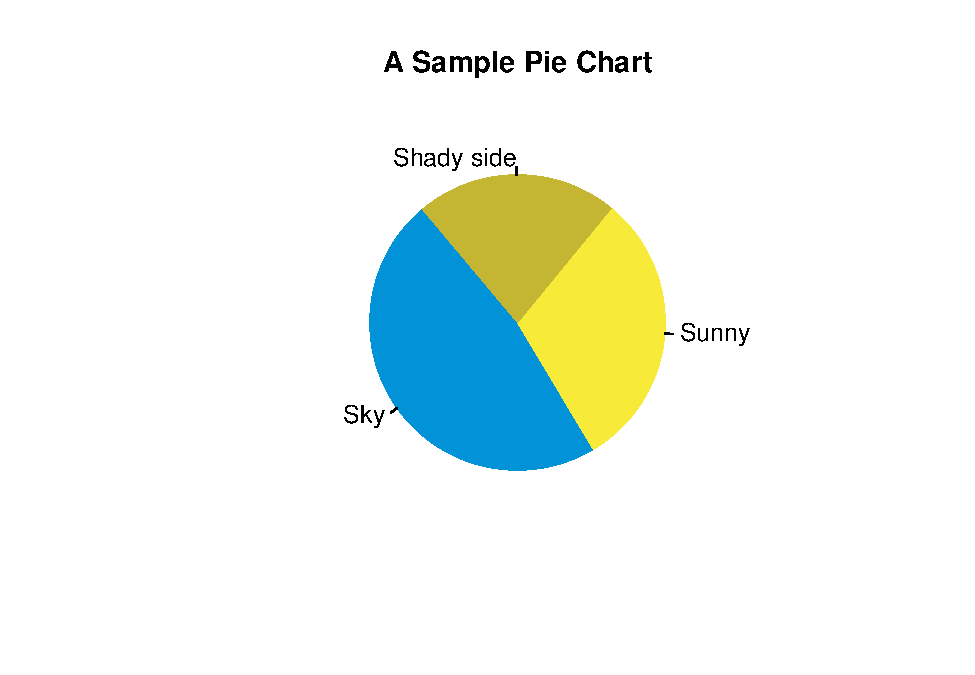
\includegraphics{03-analysis-base_files/figure-latex/unnamed-chunk-1-1.pdf}

\hypertarget{bar-chart}{%
\subsection{Bar Chart}\label{bar-chart}}

\hypertarget{chart-characteristics-color-title-axes-etc.}{%
\subsection{Chart Characteristics (color, title, axes etc.)}\label{chart-characteristics-color-title-axes-etc.}}

\hypertarget{how-to-use-proper-legends}{%
\subsection{How to Use Proper Legends?}\label{how-to-use-proper-legends}}

\hypertarget{histogram}{%
\subsection{Histogram}\label{histogram}}

\hypertarget{ogive-and-how-to-interpret-it}{%
\subsection{Ogive (and how to interpret it)}\label{ogive-and-how-to-interpret-it}}

\hypertarget{boxplot}{%
\subsection{Boxplot}\label{boxplot}}

\hypertarget{time-series-plotsline-chart}{%
\subsection{Time Series Plots/Line Chart}\label{time-series-plotsline-chart}}

\hypertarget{scatter-plot}{%
\subsection{Scatter Plot}\label{scatter-plot}}

\hypertarget{equation-and-curves}{%
\subsection{Equation and Curves}\label{equation-and-curves}}

\hypertarget{love-equation-and-curve}{%
\subsection{Love Equation and Curve}\label{love-equation-and-curve}}

\hypertarget{different-ways-of-coloring-plots}{%
\subsection{Different Ways of Coloring Plots}\label{different-ways-of-coloring-plots}}

\hypertarget{rcolorbrewer}{%
\subsubsection{RColorBrewer}\label{rcolorbrewer}}

\hypertarget{wordcloud}{%
\subsection{Wordcloud}\label{wordcloud}}

\hypertarget{comparison-of-suitability-of-plots.}{%
\subsection{Comparison of Suitability of Plots.}\label{comparison-of-suitability-of-plots.}}

\hypertarget{session-02-analysis}{%
\section{Session 02: Analysis}\label{session-02-analysis}}

Measures of Central Tendency and Dispersion (Averages, Quartiles, Variance, etc.); Correlation;

\hypertarget{tidy-1}{%
\chapter{Data Analysis: Introduction to The Tidyverse}\label{tidy-1}}

\hypertarget{reading-and-manipulating-data}{%
\section{Reading and Manipulating Data}\label{reading-and-manipulating-data}}

\hypertarget{reading-data-from-different-files}{%
\subsection{Reading Data from Different Files}\label{reading-data-from-different-files}}

\hypertarget{concept-of-tidy-data}{%
\subsection{Concept of Tidy Data}\label{concept-of-tidy-data}}

\hypertarget{how-to-make-data-tidy}{%
\subsection{How to Make Data Tidy?}\label{how-to-make-data-tidy}}

\hypertarget{subsettingfiltering-data}{%
\subsection{Subsetting/Filtering Data}\label{subsettingfiltering-data}}

\hypertarget{pipe-operator}{%
\subsection{Pipe Operator}\label{pipe-operator}}

\hypertarget{transforming-data}{%
\subsection{Transforming Data}\label{transforming-data}}

\hypertarget{summarizing-data}{%
\subsection{Summarizing Data}\label{summarizing-data}}

\hypertarget{selecting-rows-and-columns}{%
\subsection{Selecting Rows and Columns}\label{selecting-rows-and-columns}}

\hypertarget{vizualizing-data}{%
\section{Vizualizing Data}\label{vizualizing-data}}

\hypertarget{how-ggplot2-works}{%
\subsection{How ggplot2 works}\label{how-ggplot2-works}}

\hypertarget{different-geoms-and-aesthetics}{%
\subsection{Different geoms and aesthetics}\label{different-geoms-and-aesthetics}}

\hypertarget{scatter-plot}{%
\subsection{Scatter Plot}\label{scatter-plot}}

\hypertarget{bar-chart}{%
\subsection{Bar Chart}\label{bar-chart}}

\hypertarget{histogram}{%
\subsection{Histogram}\label{histogram}}

\hypertarget{boxplot}{%
\subsection{Boxplot}\label{boxplot}}

\hypertarget{time-series-plotsline-chart}{%
\subsection{Time Series Plots/Line Chart}\label{time-series-plotsline-chart}}

\hypertarget{pie-chart}{%
\subsection{Pie Chart}\label{pie-chart}}

\hypertarget{trends-within-plots}{%
\subsection{Trends within Plots}\label{trends-within-plots}}

\hypertarget{piping-output-to-ggplot2}{%
\subsection{Piping Output to ggplot2}\label{piping-output-to-ggplot2}}

\hypertarget{piping-output-to-plots}{%
\subsection{Piping Output to Plots}\label{piping-output-to-plots}}

\hypertarget{tidy-2}{%
\chapter{Advanced Tidyverse}\label{tidy-2}}

\hypertarget{advanced-visualization}{%
\section{Advanced Visualization}\label{advanced-visualization}}

\hypertarget{correlogram}{%
\subsection{Correlogram}\label{correlogram}}

\hypertarget{themes-and-legends}{%
\subsection{Themes and Legends}\label{themes-and-legends}}

\hypertarget{doughnut-chart}{%
\subsection{Doughnut Chart}\label{doughnut-chart}}

\hypertarget{density-chart}{%
\subsection{Density Chart}\label{density-chart}}

\hypertarget{violin-chart}{%
\subsection{Violin Chart}\label{violin-chart}}

\hypertarget{bubble-chart}{%
\subsection{Bubble Chart}\label{bubble-chart}}

\hypertarget{spiderradar-chart}{%
\subsection{Spider/Radar Chart}\label{spiderradar-chart}}

\hypertarget{lollipop-chart}{%
\subsection{Lollipop Chart}\label{lollipop-chart}}

\hypertarget{area-chart}{%
\subsection{Area Chart}\label{area-chart}}

\hypertarget{attaching-texts-to-plots}{%
\subsection{Attaching Texts to Plots}\label{attaching-texts-to-plots}}

\hypertarget{advanced-customization-and-attaining-what-seems-improbable}{%
\subsection{Advanced Customization And Attaining What Seems Improbable}\label{advanced-customization-and-attaining-what-seems-improbable}}

\hypertarget{animation}{%
\subsection{Animation}\label{animation}}

\hypertarget{advanced-wrangling}{%
\section{Advanced Wrangling}\label{advanced-wrangling}}

Relational Data (e.g, Merging Tables);

\hypertarget{modeling}{%
\chapter{Modeling}\label{modeling}}

\hypertarget{regression}{%
\section{Regression}\label{regression}}

\hypertarget{correlation-and-regression}{%
\subsection{Correlation and Regression}\label{correlation-and-regression}}

\hypertarget{interpretation-of-results}{%
\subsection{Interpretation of Results}\label{interpretation-of-results}}

\hypertarget{multiple-linear-regression}{%
\subsection{Multiple Linear Regression}\label{multiple-linear-regression}}

\hypertarget{regression-with-specified-intercept}{%
\subsection{Regression with Specified Intercept}\label{regression-with-specified-intercept}}

\hypertarget{choosing-between-models}{%
\subsection{Choosing between Models}\label{choosing-between-models}}

\hypertarget{poisson-regression}{%
\subsection{Poisson Regression}\label{poisson-regression}}

\hypertarget{logistic-regression}{%
\subsection{Logistic Regression}\label{logistic-regression}}

\hypertarget{prediction}{%
\subsection{Prediction}\label{prediction}}

\hypertarget{when-to-use-which-regression-with-examples}{%
\subsection{When to Use Which Regression (with Examples)}\label{when-to-use-which-regression-with-examples}}

\hypertarget{time-series-analysis}{%
\section{Time Series Analysis}\label{time-series-analysis}}

\hypertarget{test-of-hypothesis}{%
\section{Test of Hypothesis}\label{test-of-hypothesis}}

\hypertarget{confidence-interval}{%
\subsection{Confidence Interval}\label{confidence-interval}}

\hypertarget{z-test}{%
\subsection{Z-test}\label{z-test}}

\hypertarget{t-test}{%
\subsection{t-test}\label{t-test}}

\hypertarget{chi-squared-tests.}{%
\subsection{Chi-squared tests).}\label{chi-squared-tests.}}

\hypertarget{publishing}{%
\chapter{Publishing}\label{publishing}}

\hypertarget{introduction-of-markdown}{%
\section{Introduction of Markdown}\label{introduction-of-markdown}}

\hypertarget{implementation-of-rmarkdown}{%
\section{Implementation of Rmarkdown}\label{implementation-of-rmarkdown}}

\hypertarget{report-writing}{%
\subsection{Report Writing}\label{report-writing}}

\hypertarget{presentation}{%
\subsection{Presentation}\label{presentation}}

\hypertarget{books}{%
\subsection{Books}\label{books}}

  \bibliography{book.bib,packages.bib}

\end{document}
